% Options for packages loaded elsewhere
\PassOptionsToPackage{unicode}{hyperref}
\PassOptionsToPackage{hyphens}{url}
%
\documentclass[
]{book}
\usepackage{amsmath,amssymb}
\usepackage{lmodern}
\usepackage{iftex}
\ifPDFTeX
  \usepackage[T1]{fontenc}
  \usepackage[utf8]{inputenc}
  \usepackage{textcomp} % provide euro and other symbols
\else % if luatex or xetex
  \usepackage{unicode-math}
  \defaultfontfeatures{Scale=MatchLowercase}
  \defaultfontfeatures[\rmfamily]{Ligatures=TeX,Scale=1}
\fi
% Use upquote if available, for straight quotes in verbatim environments
\IfFileExists{upquote.sty}{\usepackage{upquote}}{}
\IfFileExists{microtype.sty}{% use microtype if available
  \usepackage[]{microtype}
  \UseMicrotypeSet[protrusion]{basicmath} % disable protrusion for tt fonts
}{}
\makeatletter
\@ifundefined{KOMAClassName}{% if non-KOMA class
  \IfFileExists{parskip.sty}{%
    \usepackage{parskip}
  }{% else
    \setlength{\parindent}{0pt}
    \setlength{\parskip}{6pt plus 2pt minus 1pt}}
}{% if KOMA class
  \KOMAoptions{parskip=half}}
\makeatother
\usepackage{xcolor}
\IfFileExists{xurl.sty}{\usepackage{xurl}}{} % add URL line breaks if available
\IfFileExists{bookmark.sty}{\usepackage{bookmark}}{\usepackage{hyperref}}
\hypersetup{
  hidelinks,
  pdfcreator={LaTeX via pandoc}}
\urlstyle{same} % disable monospaced font for URLs
\usepackage{longtable,booktabs,array}
\usepackage{calc} % for calculating minipage widths
% Correct order of tables after \paragraph or \subparagraph
\usepackage{etoolbox}
\makeatletter
\patchcmd\longtable{\par}{\if@noskipsec\mbox{}\fi\par}{}{}
\makeatother
% Allow footnotes in longtable head/foot
\IfFileExists{footnotehyper.sty}{\usepackage{footnotehyper}}{\usepackage{footnote}}
\makesavenoteenv{longtable}
\usepackage{graphicx}
\makeatletter
\def\maxwidth{\ifdim\Gin@nat@width>\linewidth\linewidth\else\Gin@nat@width\fi}
\def\maxheight{\ifdim\Gin@nat@height>\textheight\textheight\else\Gin@nat@height\fi}
\makeatother
% Scale images if necessary, so that they will not overflow the page
% margins by default, and it is still possible to overwrite the defaults
% using explicit options in \includegraphics[width, height, ...]{}
\setkeys{Gin}{width=\maxwidth,height=\maxheight,keepaspectratio}
% Set default figure placement to htbp
\makeatletter
\def\fps@figure{htbp}
\makeatother
\setlength{\emergencystretch}{3em} % prevent overfull lines
\providecommand{\tightlist}{%
  \setlength{\itemsep}{0pt}\setlength{\parskip}{0pt}}
\setcounter{secnumdepth}{-\maxdimen} % remove section numbering
\ifLuaTeX
  \usepackage{selnolig}  % disable illegal ligatures
\fi

\author{}
\date{}

\begin{document}
\frontmatter

\mainmatter
\hypertarget{in-vitro-transcription-pf-pfc8-plasmid}{%
\chapter{\texorpdfstring{\emph{In vitro} transcription pf pFC8
plasmid}{In vitro transcription pf pFC8 plasmid}}\label{in-vitro-transcription-pf-pfc8-plasmid}}

\hypertarget{reagents}{%
\section{Reagents}\label{reagents}}

\begin{longtable}[]{@{}ll@{}}
\toprule
Name & Volume (ul) \\
\midrule
\endhead
5x Buffer & 4 \\
100 mM DTT & 4 \\
2.5 mM NTP & 1 \\
DNA & 2.12 \\
H20 & 8.88 \\
\bottomrule
\end{longtable}

DNA concentration much lower than was marked on the tube.

\hypertarget{samples}{%
\section{Samples}\label{samples}}

\begin{itemize}
\tightlist
\item
  Control: Master mix only, no transcription
\item
  Transcribed: Master mix + T7 Polymerase + RNAaseA
\item
  Transcribed + RNAase H: Master mix + T7 + RNAaseA Polymerase + RNAaseH
\end{itemize}

\hypertarget{protocol-notes}{%
\section{Protocol notes}\label{protocol-notes}}

\begin{enumerate}
\def\labelenumi{\arabic{enumi}.}
\tightlist
\item
  Measure DNA concentration using Nanodrop
\item
  Calculate volume of DNA sample required for \textasciitilde{} 200 ng
  per lane
\item
  Make master mix
\item
  Aliquot 5 ul for control and remaining sample into PCR reaction tubes.
\item
  Create thermocycler reaction profile; 37 C for 20 mins then 65 C for
  10 mins.
\item
  Add 0.5 ul T7 Polymerase to the treatment tube (15 ul master mix). Run
  thermocycler profile.
\item
  Prepare 0.9 \% agarose gel using 40 ml TBE buffer while thermocycler
  is running.
\item
  Add 0.5 ul RNAaseA to treatment tube incubate in thermocycler for 20
  mins at 37 C.
\item
  Split treatment tube in half (7.5 ul remove to third PCR tube) and add
  0.5 ml RNAaseH to the third sample.
\item
  Incubate at 37 C for 20 mins.
\item
  Add protease K to all samples to eat junk and incubate at 37 C for 10
  mins.
\item
  Load samples into gel using purple loading dye.
\item
  Run get for 1 hr at 90 volts.
\item
  Remove gel from tray and place into temporary container (tuperware
  will work) and add 1 ul of ethedium bromide and aggitate on the
  spinner machine by the gel imager for at least 10 minutes.
\item
  Image the gel and pray.
\end{enumerate}

\hypertarget{results}{%
\section{Results}\label{results}}

Not great lol. Somehow it looks like the DNA did not make it onto the
gel.

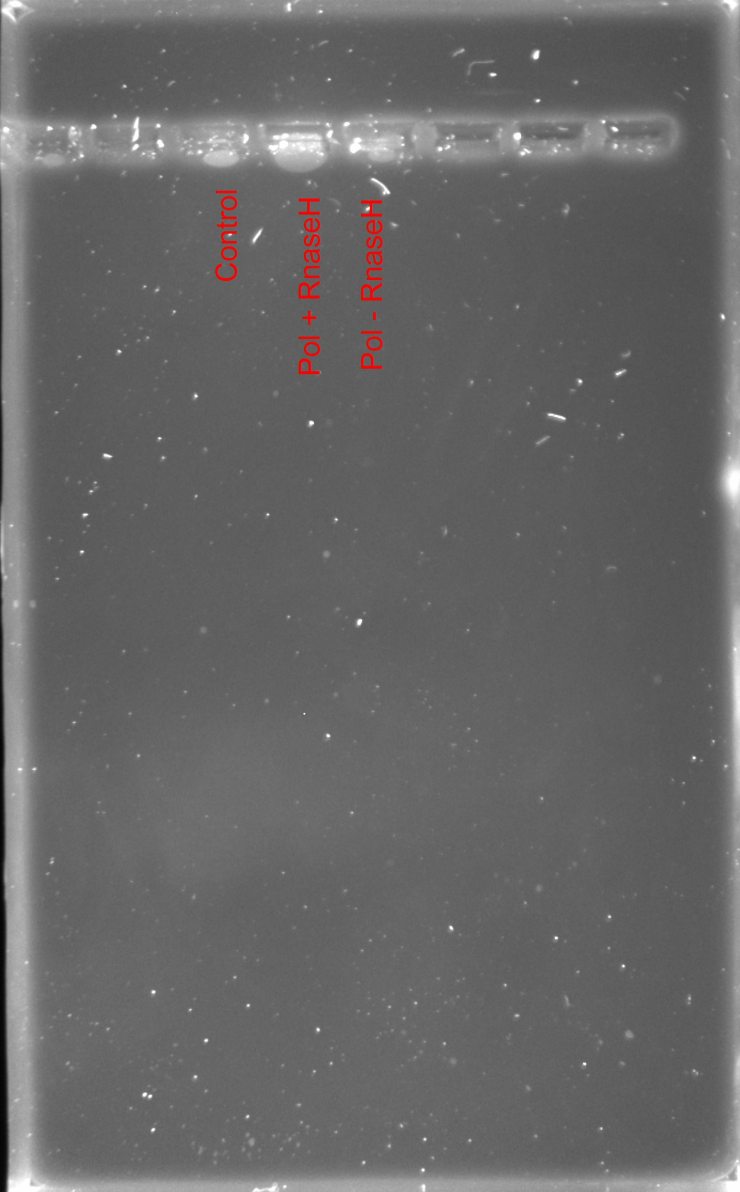
\includegraphics{images/ivt_4-6-2020.png}

\hypertarget{ivt-plasmid-pfc8-t1-t2}{%
\chapter{IVT Plasmid pFC8 T1 T2}\label{ivt-plasmid-pfc8-t1-t2}}

\hypertarget{summary}{%
\section{Summary}\label{summary}}

Redoing the IVT assay with different batch of the plasmid.

\hypertarget{reagents-1}{%
\section{Reagents}\label{reagents-1}}

\begin{longtable}[]{@{}ll@{}}
\toprule
Name & Volume (ul) \\
\midrule
\endhead
5x Buffer & 4 \\
100 mM DTT & 4 \\
2.5 mM NTP & 1 \\
DNA & 4 \\
H20 & 11 \\
\bottomrule
\end{longtable}

\hypertarget{protocol-flow}{%
\section{Protocol Flow}\label{protocol-flow}}

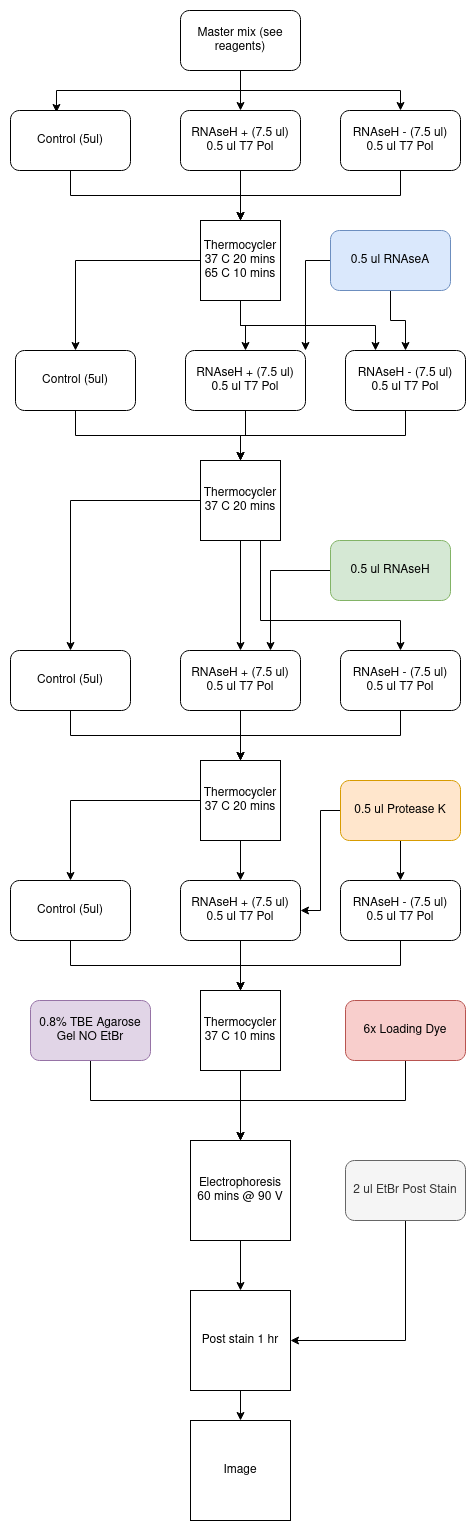
\includegraphics{images/IVT_4-15-21.png}

Note: When using more plasmids do not split the RNAse + and - cases
until after the polymerase is added. Can keep these in one tube until
then.

\hypertarget{results-1}{%
\section{Results}\label{results-1}}

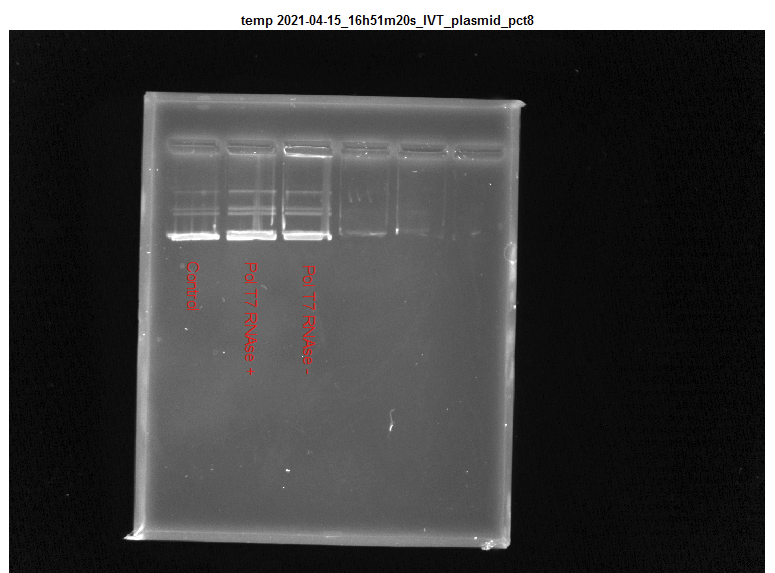
\includegraphics{images/IVT_4-15-21_gel.png}

There is actually DNA this time but no band shifting :(

\backmatter
\end{document}
